\documentclass[journal,12pt,twocolumn]{IEEEtran}
%
\usepackage{setspace}
\usepackage{gensymb}
%\doublespacing
\singlespacing

%\usepackage{graphicx}
%\usepackage{amssymb}
%\usepackage{relsize}
\usepackage[cmex10]{amsmath}
%\usepackage{amsthm}
%\interdisplaylinepenalty=2500
%\savesymbol{iint}
%\usepackage{txfonts}
%\restoresymbol{TXF}{iint}
%\usepackage{wasysym}
\usepackage{amsthm}
%\usepackage{iithtlc}
\usepackage{mathrsfs}
\usepackage{txfonts}
\usepackage{stfloats}
\usepackage{bm}
\usepackage{cite}
\usepackage{cases}
\usepackage{subfig}
%\usepackage{xtab}
\usepackage{longtable}
\usepackage{multirow}
%\usepackage{algorithm}
%\usepackage{algpseudocode}
\usepackage{enumitem}
\usepackage{mathtools}
\usepackage{steinmetz}
\usepackage{tikz}
\usepackage{circuitikz}
\usepackage{verbatim}
\usepackage{tfrupee}
\usepackage[breaklinks=true]{hyperref}
%\usepackage{stmaryrd}
\usepackage{tkz-euclide} % loads  TikZ and tkz-base
%\usetkzobj{all}
\usetikzlibrary{calc,math}
\usepackage{listings}
    \usepackage{color}                                            %%
    \usepackage{array}                                            %%
    \usepackage{longtable}                                        %%
    \usepackage{calc}                                             %%
    \usepackage{multirow}                                         %%
    \usepackage{hhline}                                           %%
    \usepackage{ifthen}                                           %%
  %optionally (for landscape tables embedded in another document): %%
    \usepackage{lscape}     
\usepackage{multicol}
\usepackage{chngcntr}
%\usepackage{enumerate}

%\usepackage{wasysym}
%\newcounter{MYtempeqncnt}
\DeclareMathOperator*{\Res}{Res}
%\renewcommand{\baselinestretch}{2}
\renewcommand\thesection{\arabic{section}}
\renewcommand\thesubsection{\thesection.\arabic{subsection}}
\renewcommand\thesubsubsection{\thesubsection.\arabic{subsubsection}}

\renewcommand\thesectiondis{\arabic{section}}
\renewcommand\thesubsectiondis{\thesectiondis.\arabic{subsection}}
\renewcommand\thesubsubsectiondis{\thesubsectiondis.\arabic{subsubsection}}

% correct bad hyphenation here
\hyphenation{op-tical net-works semi-conduc-tor}
\def\inputGnumericTable{}                                 %%

\lstset{
%language=C,
frame=single, 
breaklines=true,
columns=fullflexible
}
%\lstset{
%language=tex,
%frame=single, 
%breaklines=true
%}

\begin{document}
%


\newtheorem{theorem}{Theorem}[section]
\newtheorem{problem}{Problem}
\newtheorem{proposition}{Proposition}[section]
\newtheorem{lemma}{Lemma}[section]
\newtheorem{corollary}[theorem]{Corollary}
\newtheorem{example}{Example}[section]
\newtheorem{definition}[problem]{Definition}
%\newtheorem{thm}{Theorem}[section] 
%\newtheorem{defn}[thm]{Definition}
%\newtheorem{algorithm}{Algorithm}[section]
%\newtheorem{cor}{Corollary}
\newcommand{\BEQA}{\begin{eqnarray}}
\newcommand{\EEQA}{\end{eqnarray}}
\newcommand{\define}{\stackrel{\triangle}{=}}
\bibliographystyle{IEEEtran}
%\bibliographystyle{ieeetr}
\providecommand{\mbf}{\mathbf}
\providecommand{\pr}[1]{\ensuremath{\Pr\left(#1\right)}}
\providecommand{\qfunc}[1]{\ensuremath{Q\left(#1\right)}}
\providecommand{\sbrak}[1]{\ensuremath{{}\left[#1\right]}}
\providecommand{\lsbrak}[1]{\ensuremath{{}\left[#1\right.}}
\providecommand{\rsbrak}[1]{\ensuremath{{}\left.#1\right]}}
\providecommand{\brak}[1]{\ensuremath{\left(#1\right)}}
\providecommand{\lbrak}[1]{\ensuremath{\left(#1\right.}}
\providecommand{\rbrak}[1]{\ensuremath{\left.#1\right)}}
\providecommand{\cbrak}[1]{\ensuremath{\left\{#1\right\}}}
\providecommand{\lcbrak}[1]{\ensuremath{\left\{#1\right.}}
\providecommand{\rcbrak}[1]{\ensuremath{\left.#1\right\}}}
\theoremstyle{remark}
\newtheorem{rem}{Remark}
\newcommand{\sgn}{\mathop{\mathrm{sgn}}}
\providecommand{\abs}[1]{\left\vert#1\right\vert}
\providecommand{\res}[1]{\Res\displaylimits_{#1}} 
\providecommand{\norm}[1]{\left\lVert#1\right\rVert}
%\providecommand{\norm}[1]{\lVert#1\rVert}
\providecommand{\mtx}[1]{\mathbf{#1}}
\providecommand{\mean}[1]{E\left[ #1 \right]}
\providecommand{\fourier}{\overset{\mathcal{F}}{ \rightleftharpoons}}
%\providecommand{\hilbert}{\overset{\mathcal{H}}{ \rightleftharpoons}}
\providecommand{\system}{\overset{\mathcal{H}}{ \longleftrightarrow}}
	%\newcommand{\solution}[2]{\vec{Solution:}{#1}}
\newcommand{\solution}{\noindent \vec{Solution: }}
\newcommand{\cosec}{\,\text{cosec}\,}
\providecommand{\dec}[2]{\ensuremath{\overset{#1}{\underset{#2}{\gtrless}}}}
\newcommand{\myvec}[1]{\ensuremath{\begin{pmatrix}#1\end{pmatrix}}}
\newcommand{\mydet}[1]{\ensuremath{\begin{vmatrix}#1\end{vmatrix}}}
%\numberwithin{equation}{section}
\numberwithin{equation}{subsection}
%\numberwithin{problem}{section}
%\numberwithin{definition}{section}
\makeatletter
\@addtoreset{figure}{problem}
\makeatother
\let\StandardTheFigure\thefigure
\let\vec\mathbf
%\renewcommand{\thefigure}{\theproblem.\arabic{figure}}
\renewcommand{\thefigure}{\theproblem}
%\setlist[enumerate,1]{before=\renewcommand\theequation{\theenumi.\arabic{equation}}
%\counterwithin{equation}{enumi}
%\renewcommand{\theequation}{\arabic{subsection}.\arabic{equation}}
\def\putbox#1#2#3{\makebox[0in][l]{\makebox[#1][l]{}\raisebox{\baselineskip}[0in][0in]{\raisebox{#2}[0in][0in]{#3}}}}
     \def\rightbox#1{\makebox[0in][r]{#1}}
     \def\centbox#1{\makebox[0in]{#1}}
     \def\topbox#1{\raisebox{-\baselineskip}[0in][0in]{#1}}
     \def\midbox#1{\raisebox{-0.5\baselineskip}[0in][0in]{#1}}
\vspace{3cm}
\title{ASSIGNMENT 3}
\author{YENIGALLA SAMYUKTHA\\EE20MTECH14019}
%
\maketitle
\newpage
%\tableofcontents
\bigskip
\renewcommand{\thefigure}{\theenumi}
\renewcommand{\thetable}{\theenumi}
%
\begin{abstract}
This document proves that triangles on the same base and having equal areas lie between the same parallel lines.
\end{abstract}
Download latex-tikz codes from 
%
\begin{lstlisting}
https://github.com/EE20MTECH14019/EE5609/tree/master/Assignment_3
\end{lstlisting}
%
\section{Problem}
\item Triangles on the same base (or equal bases) and having equal areas lie between the same parallels.
\section{Explanation}
\item Consider $\vec{A},\vec{B},\vec{C}$ are three points of a triangle $\triangle ABC$, $\vec{D}, \vec{B}, \vec{C}$ are three points of another triangle $\triangle DBC$, both triangles having same base BC and $\vec{B}$ at origin, 
\begin{align}
    \label{1}
    \vec{A}-\vec{B}=\vec{A}\\
    \label{2}
    \vec{C}-\vec{B}=\vec{C}\\
    \label{3}
    \vec{D}-\vec{B}=\vec{D}
\end{align}
\item The area of the triangle $\triangle ABC$ is,
\begin{align}
    \label{4}
    Area\brak{\triangle ABC} = \frac{1}{2}\norm{\brak{\vec{A} - \vec{B}} \times \brak{\vec{C} - \vec{B}}}
\end{align}
\item Substituting \eqref{1} and \eqref{2} in \eqref{4}, 
\begin{align}
    \label{ABC}
    \implies Area\brak{\triangle ABC} = \frac{1}{2}\norm{\brak{\vec{A} \times \vec{C}}}
\end{align}
% figure
\begin{figure}[!ht] \label{fig:triangle_abc}
\centering
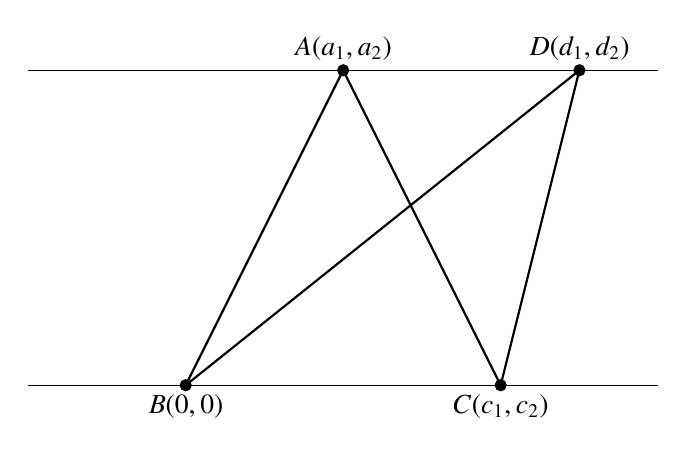
\begin{tikzpicture}
\draw (-2,0) -- (6,0); 
\draw (-2,4) -- (6,4);
\filldraw[black] (0,0) circle (2pt) node[anchor=north] {$B (0,0)$};
\filldraw[black] (2,4) circle (2pt) node[anchor=south] {$A (a_1,a_2)$};
\filldraw[black] (4,0) circle (2pt) node[anchor=north] {$C (c_1,c_2)$};
\filldraw[black] (5,4) circle (2pt) node[anchor=south] {$D (d_1,d_2)$};
\draw[black,thick] (0,0) -- (2,4);
\draw[black,thick] (4,0) -- (2,4);
\draw[black,thick] (0,0) -- (5,4);
\draw[black,thick] (4,0) -- (5,4);
\draw[black] (4,0) -- (0,0);
\end{tikzpicture}
\caption{$\triangle ABC$ and $\triangle DBC$ with BC as common base}
\label{fig:solutions/1/2/two}
\end{figure}
\item The area of the triangle $\triangle DBC$ is,
\begin{align}
    \label{5}
    Area\brak{\triangle ABC} = \frac{1}{2}\norm{\brak{\vec{D} - \vec{B}} \times \brak{\vec{C} - \vec{B}}}
\end{align}   
\item Substituting \eqref{2} and \eqref{3} in \eqref{5}, 
\begin{align}
    \label{DBC}
    \implies Area\brak{\triangle DBC} = \frac{1}{2}\norm{\brak{\vec{D} \times \vec{C}}}
\end{align}
\item Given the area of $\triangle ABC$ is equal to the area $\triangle DBC$, from equations \eqref{ABC} and \eqref{DBC}
\begin{align}
    \label{modeq}
    \frac{1}{2}\norm{\brak{\vec{A} \times \vec{C}}} = \frac{1}{2}\norm{\brak{\vec{D} \times \vec{C}}}
\end{align}
Squaring on both sides of the equation \eqref{modeq}, we get
\begin{align}
    \norm{\brak{\vec{A} \times \vec{C}}}^2 = \norm{\brak{\vec{D} \times \vec{C}}}^2
\end{align}
\begin{align}
    \implies\brak{\vec{A}\times\vec{C}}^T \brak{\vec{A}\times\vec{C}} = \brak{\vec{D}\times\vec{C}}^T \brak{\vec{D}\times\vec{C}}
\end{align}
\begin{equation}
\begin{align}
    \implies \brak{\vec{A}^T\vec{A}}\brak{\vec{C}^T\vec{C}} - \brak{\vec{A}^T\vec{C}}\brak{\vec{C}^T\vec{A}} =\\ \brak{\vec{D}^T\vec{D}}\brak{\vec{C}^T\vec{C}} - \brak{\vec{D}^T\vec{C}}\brak{\vec{C}^T\vec{D}}
\end{align}
\end{equation}
\begin{align}
    \label{eq11}
    \implies\norm{\vec{A}}^2\norm{\vec{C}}^2 - \brak{\vec{A}^T\vec{C}}^2 = \norm{\vec{D}}^2\norm{\vec{C}^2} - \brak{\vec{D}^T\vec{C}}^2 
\end{align}
Let $\vec{A}=\myvec{a1\\a2}$, $\vec{C}=\myvec{c_1\\0}$ and $\vec{D}=\myvec{d_1\\d_2}$ .Then equation \eqref{eq11} can be written as,
\begin{align}
    \label{lbo}
    \brak{a_1^2+a_2^2}\brak{c_1^2}-\brak{a_1c_1}^2 = \brak{d_1^2+d_2^2}\brak{c_1^2} - \brak{d_1c_1}^2
\end{align}
\begin{align}
    \implies a_2 = d_2
\end{align}
Now we have,
\begin{align}
    \label{eq14}
    \brak{\vec{D}-\vec{A}}=\myvec{d_1-a_1\\d_2-a_2} = \myvec{d_1-a_1\\0}\\ 
    \label{eq15}
    \brak{\vec{C}-\vec{B}} = \myvec{c_1-0 \\ 0-0} = \myvec{c_1 \\ 0}
\end{align}
From equations \eqref{eq14} and \eqref{eq15}, we can say
\begin{align}
    \brak{\vec{D}-\vec{A}}=\frac{d_1-a_1}{c_1}\brak{\vec{C}-\vec{B}}\\
    \label{lst}
    \implies \brak{\vec{D}-\vec{A}}=k\brak{\vec{C}-\vec{B}}
\end{align}
where $k$ is a constant. From the equation \eqref{lst}, we can say that $AD \parallel BC$. Hence the two triangles $\triangle ABC$ and $\triangle DBC$ lie between the same parallels AD and BC
\end{document}
